\chapter{Beliebig veränderliche Felder}
Im Folgenden werden die \textbf{Maxwell-Gleichungen} ($\nearrow$\ref{ind},\ref{quellf},\ref{durchf},\ref{gauss}) \textbf{ohne Einschränkung} betrachtet, d.h. es wird kein Term mehr vernachlässigt. In der Regel werden auch in diesem Kapitel \textbf{homogene, lineare und isotrope} Medien betrachtet. Das bedeutet, dass die Materialgleichungen in der vereinfachten Form wie in Gleichung \ref{matlinhomis} gelten. Ferner wird vereinfachend angenommen, dass lokal das \textbf{ohmsche Gesetz} nach Gleichung \ref{ohm} gilt (also in Leitern die Kraftwirkung auf Ladungsträger herrührend vom $B$-Feld vernachlässigbar ist). 
 \section{Ladungserhaltung}
 In \ref{ladungserhaltung} wurde die \textbf{Ladungserhaltung} als axiomatisch vorausgesetzt und davon ausgehend auf die Maxwell-Gleichungen geschlossen. Das funktioniert auch umgekehrt, die Kontinuitätsgleichung  ($\nearrow$\ref{kont}) lässt sich, wie in \ref{kontherl} gezeigt wurde, aus \ref{durchf}, \ref{gauss} und \ref{divrot} herleiten. Die Kontinuitätsgleichung ist ein Ausdruck der Ladungserhaltung.
\section{Energieerhaltung (Poyntingscher Satz)}
\subsection{Differentielle Form des Poyntingschen Satzes}
Zur konzeptionellen Herleitung der Verlustleistungsdichte wird zunächst eine bewegte Ladung $\dd q = \rho_\text{V}\dd V$, welche sich gleichförmig mit der Geschwindigkeit $\vec{v}$ ($|\vec{v}| \ll c$) in homogenen Feldern bewegt betrachtet. Nach \ref{lorentz} wirkt auf die Ladung eine Lorentzkraft:
		        \begin{equation}\begin{split}
				        \vec{F} = q \left( \vec{E} + \vec{v} \times \vec{B} \right) \implies \dd\vec{F} = \rho_\text{V}\dd V \left( \vec{E} + \vec{v} \times \vec{B} \right)
			        \end{split}\end{equation}
Aus der Kraft lässt sich die differentiell \textbf{verrichtete Arbeit} $\dd W$ bei Verschiebung um $\Delta\vec{s} = \vec{v} \Delta t$ ($\Rightarrow\Delta\vec{s} \parallel \vec{v}$, linearer Zusammenhang wegen gleichförmiger Bewegung) bestimmen:
		        \begin{equation}\begin{split}
				        \dd W =  \dd\vec{F} \cdot \Delta\vec{s} = \rho_\text{V}\dd V \left( \vec{E} + \vec{v} \times \vec{B} \right)\cdot \Delta\vec{s}
				        = \rho_\text{V}\dd V\, \vec{E} \cdot \Delta\vec{s} = \rho_\text{V}\dd V\, \vec{E} \cdot \vec{v} \Delta t
			        \end{split}\end{equation}
Außerdem folgt die differentielle \textbf{Leistung} $\dd\left( \frac{W}{\Delta t}\right)$ ($\nearrow$\ref{ladunggeschw}, $v\leftrightarrow v_\text{D}$):
		        \begin{equation}\begin{split}
				        \dd\left( \frac{W}{\Delta t}\right) = \rho_\text{V}\vec{v}\cdot\vec{E}\, \dd V = \vec{J}\cdot\vec{E}\, \dd V
			        \end{split}\end{equation}
Hiermit ergibt sich die \textbf{Leistung} zu:
		        \begin{equation}\begin{split}
				        P = \frac{W}{\Delta t} = \iiint\limits_V \vec{J}\cdot\vec{E}\, \dd V \text{ (analog zu } P=U\cdot I \text{ im Leiter)}
			        \end{split}\end{equation}
Die Analogie gilt nur, wenn $E$ ein konservatives Feld ist. Nur dann ist die Einführung einer Spannung sinnvoll. Für die \textbf{Verlustleistungsdichte} gilt ($\nearrow$\ref{verlustleist},\ref{durchf}):
\begin{equation}\begin{split}
				        p_\text{V} =\frac{\partial w_\text{mech}}{\partial t}= \vec{J}\cdot\vec{E} = \vec{E} \cdot \vec{J} = \vec{E} \cdot \left(\rot \vec{H}  - \frac{\partial \vec{D} }{\partial t}\right) =  \textcolor{red}{\vec{E} \cdot \rot \vec{H} } - \vec{E} \cdot \frac{\partial \vec{D} }{\partial t}
			    \end{split}\end{equation}
		 Der rote Term ist bei weitergehenden Rechnungen störend, also soll er eliminiert werden ($\nearrow$\ref{divcross}):
		        \begin{equation}\begin{split}
				        \div \left(\vec{E} \times \vec{H} \right) = \vec{H} \cdot\rot \vec{E} - \textcolor{red}{\vec{E} \cdot \rot \vec{H} } = - \vec{H} \cdot\frac{\partial \vec{B} }{\partial t} - \textcolor{red}{\vec{E} \cdot \rot \vec{H} }
			        \end{split}\end{equation}
	Somit ergibt sich der \textbf{Poyntingsche Satz} in differentieller Form \textbf{allgemein} zu:
		        \begin{equation}\label{poyntsat}\begin{split}
				        \boxed{\frac{\partial w_\text{mech}}{\partial t}=\vec{E} \cdot \vec{J} = - \div \left(\vec{E} \times \vec{H} \right) - \vec{H} \cdot\frac{\partial \vec{B} }{\partial t} - \vec{E} \cdot \frac{\partial \vec{D} }{\partial t} } 
			        \end{split}\end{equation}
		   Für \textbf{homogene, lineare und isotrope Medien} folgt ($\nearrow$\ref{matlinhomis}):
		        \begin{equation}\label{poyntsathli1}\begin{split}
		        		\frac{1}{2}\frac{\partial}{\partial t}\left(\vec{H} \cdot\vec{B}\right) &= \frac{1}{2}\left(\frac{\partial}{\partial t}\vec{H} \cdot\vec{B} + \vec{H} \cdot\frac{\partial}{\partial t}\vec{B}\right)= \frac{\mu}{2}\left(\frac{\partial}{\partial t}\vec{H} \cdot\vec{H} + \vec{H} \cdot\frac{\partial}{\partial t}\vec{H}\right)=\vec{H}\cdot\frac{\partial}{\partial t}\vec{B}\\
				        \Rightarrow\quad\vec{E} \cdot \vec{J} &= - \div \left(\vec{E} \times \vec{H} \right) - \frac{\partial}{\partial t}\left[\frac{1}{2} \vec{H} \cdot\vec{B}  + \frac{1}{2} \vec{E} \cdot \vec{D} \right] 
			        \end{split}\end{equation}
		   In diesem Ausdruck kommen die magnetische und elektrische Energiedichte vor ($\nearrow$\ref{edichteE},\ref{edichteH}). Es wird die \textbf{elektromagnetische Energiedichte} eingeführt:
		   \begin{equation}
		   	\boxed{w_\text{em}=w_\text{e}+w_\text{m}=\frac{1}{2} \vec{H} \cdot\vec{B}  + \frac{1}{2} \vec{E} \cdot \vec{D}}
		   \end{equation}
		   Damit lässt sich für \textbf{homogene, lineare und isotrope Medien} \ref{poyntsathli1} folgendermaßen schreiben:
		        \begin{equation}\label{poyntsathli}\begin{split}
				     \boxed{ \frac{\partial w_\text{mech}}{\partial t}=\vec{E} \cdot \vec{J}= - \div \left(\vec{E} \times \vec{H} \right) - \frac{\partial w_\text{em}}{\partial t}}
			        \end{split}\end{equation}
		   \subsection{Integrale Form des Poyntingschen Satzes}
		   Der Übergang zur integralen Darstellung erfolgt über ein Volumenintegral:
		        \begin{align*}
			         \iiint\limits_V \vec{E} \cdot \vec{J} \dd V & = - \oiint\limits_{O(V)} \vec{E} \times \vec{H}  \cdot \dd\vec{A} - \frac{\partial}{\partial t} \iiint\limits_V w_\text{em} \dd V \\
			         \underbrace{\frac{\partial}{\partial t} \iiint\limits_V w_\text{mech} \dd V }_{\text{mechanisch, thermodynamisch}}                                                       & = \underbrace{- \oiint\limits_{O(V)} \vec{E} \times \vec{H}  \cdot \dd\vec{A} - \frac{\partial}{\partial t} \iiint\limits_V w_\text{em} \dd V         }_\text{elektromagnetisch}                 
			    \end{align*}
			   Es folgt der \textbf{integrale Poyntigscher Satz} für \textbf{homogene, lineare und isotrope Medien}:
			    \begin{equation}\label{poyntint}
			        \boxed{\frac{\partial}{\partial t} \iiint\limits_V \left( w_\text{mech} + w_\text{em} \right) \dd V                                  = - \oiint\limits_{O(V)} \vec{E} \times \vec{H}  \cdot \dd\vec{A}}
		        \end{equation}
  \subsection{Poynting-Vektor}
		  Änderung der Energie im Volumen $V$ entspricht nach \ref{poyntint} dem Fluss des Vektors $\vec{S}= \vec{E} \times \vec{H} $ durch die Oberfläche des Volumens $O(V)$. Das ist anschaulich eine Formulierung der Energieerhaltung.
		   Die Größe
		        \begin{equation}\begin{split}
				        \boxed{\vec{S}= \vec{E} \times \vec{H} } 
			        \end{split}\end{equation}
		        ist die lokale \textbf{Energieflussdichte} oder der \textbf{Poynting-Vektor}.
		   Hiermit schreiben sich integraler und differentieller Poyntingscher Satz nach \ref{poyntint} und \ref{poyntsathli} wie folgt:
		        \begin{align}
			        \frac{\partial}{\partial t} \iiint\limits_V \left( w_\text{mech} + w_\text{em} \right) \dd V + \oiint\limits_{O(V)} \vec{S} \cdot \dd\vec{A} & = 0 \\
			        \frac{\partial}{\partial t} \left( w_\text{mech} + w_\text{em} \right) + \div \vec{S}                                                        & =0
		    \end{align}
  \subsection{Formulierung bei harmonischer Zeitabhängigkeit}
  \subsubsection{Frequenzbereich}
  Bei harmonischer Zeitabhängigkeit ist wie bei den quasistationären Feldern eine Darstellung im Frequenzbereich vorteilhaft ($\nearrow$\ref{frequenzbereich}). Die harmonische Zeitabhängigkeit stellt keine Einschränkung dar, im Sinne einer Fourier-Synthese kann man durch harmonische Signale verschiedener Frequenz ein beliebiges Signal darstellen. Es gilt:		        \begin{equation}\begin{split}
				        \vec{E}(\vec{r} ,\,t) = \re{\ubar{\vec{E}}(\vec{r} )   \mathrm{e}^{\mathrm{j} \omega  t} } = \frac{1}{2} \left[\ubar{\vec{E}}(\vec{r} )   \mathrm{e}^{\mathrm{j} \omega  t}  + \ubar{\vec{E}}^\star(\vec{r} )   \mathrm{e}^{-\mathrm{j} \omega  t}  \right]
			        \end{split}\end{equation}
 Die Energiedichte $w_\text{e} = \frac{1}{2} \vec{E} \cdot \vec{D} $ lässt sich beispielsweise folgendermaßen schreiben:
		        \begin{equation}\begin{split}
				        w_\text{e} &= \frac{1}{2} \vec{E} \cdot \vec{D}  \\
				        &= \frac{1}{2} \left[ \frac{1}{2} \left(\ubar{\vec{E}}   \mathrm{e}^{\mathrm{j} \omega  t}  + \ubar{\vec{E}}^\star   \mathrm{e}^{-\mathrm{j} \omega  t}  \right)\right] \cdot \left[ \frac{1}{2} \left(\vec{\ubar{D}}   \mathrm{e}^{\mathrm{j} \omega  t}  + \vec{\ubar{D}}^\star   \mathrm{e}^{-\mathrm{j} \omega  t}  \right)  \right] \\
				        &= \frac{1}{8} \left[ \ubar{\vec{E}} \cdot \vec{\ubar{D}}   \mathrm{e}^{\mathrm{j} 2\omega  t} + \ubar{\vec{E}}^\star \cdot \vec{\ubar{D}}^\star   \mathrm{e}^{-\mathrm{j} 2\omega  t}\right] +  \frac{1}{8} \left[ \ubar{\vec{E}} \cdot \vec{\ubar{D}}^\star  + \ubar{\vec{E}}^\star \cdot \vec{\ubar{D}} \right]\\
				        &=\frac{1}{4}\re{\ubar{\vec{E}} \cdot \vec{\ubar{D}}   \mathrm{e}^{\mathrm{j} 2\omega  t}} + \frac{1}{4}\re{\ubar{\vec{E}} \cdot \vec{\ubar{D}}^\star}
			        \end{split}\end{equation}
		        $w_\text{e} = \frac{1}{2} \vec{E} \cdot \vec{D} \neq  \frac{1}{2} \vec{\ubar{E}} \cdot \vec{\ubar{D}}$, weil die Multiplikation nicht linear ist ($\nearrow$\ref{ansig}). Damit man im Zeit- und Bildbereich äquivalent rechnen kann, dürfen nur lineare Operationen ausgeführt werden.
  \subsubsection{Mittelwerte und komplexer Poynting-Vektor}
	  Für den die zeitlichen Mittelwerte gilt (da es sich um periodische Größen handelt reicht die Mittlung über eine Periode):
		        \begin{align}
			        \langle w_\text{e} \rangle    & = \frac{1}{4}\re{\ubar{\vec{E}} \cdot \vec{\ubar{D}}^\star} \stackrel{(\vec{D} =\varepsilon\vec{E}), \varepsilon\in \mathbb{R}}{=} \frac{1}{4}\ubar{\vec{E}} \cdot \vec{\ubar{D}}^\star \label{kompledichtmag}\\
			        \langle w_\text{m} \rangle    & = \frac{1}{4}\re{\vec{\ubar{H}} \cdot \vec{\ubar{B}}^\star} \stackrel{(\vec{B} =\mu\vec{H} ), \mu\in \mathbb{R}}{=} \frac{1}{4}\vec{\ubar{H}} \cdot \vec{\ubar{B}}^\star                \label{komplmdichtmag}\\
			        \langle p_\text{V} \rangle    & = \frac{1}{2}\re{\ubar{\vec{E}} \cdot \ubar{\vec{J}}^\star} \stackrel{(\vec{J}=\kappa\vec{E}), \kappa\in \mathbb{R}  }{=}\frac{1}{2}\ubar{\vec{E}} \cdot \ubar{\vec{J}}^\star       \\
			        \langle \vec{S}\rangle & = \frac{1}{2}\re{\ubar{\vec{E}} \times \vec{\ubar{H}}^\star} = \re{\vec{\ubar{S}}} \label{komplpoyntmit}
		\end{align}
		   Hierbei wird der \textbf{komplexe Poyntingsche Vektor} $\vec{\ubar{S}}$ eingeführt:
		        \begin{equation}\begin{split}
				        \boxed{\vec{\ubar{S}} = \frac{1}{2}\ubar{\vec{E}} \times \vec{\ubar{H}}^\star} {\color{blue}=\ubar{\vec{E}} \times \vec{\ubar{H}}^\star \quad\text{mit RMS-Zeigern}}
			        \end{split}\end{equation}
		     
  \subsubsection{Komplexer Poyntingscher-Satz in differentieller Form}
		  Zunächst wird die Divergenz des komplexen Poynting-Vektors gebildet ($\nearrow$\ref{divcross},\ref{ind},\ref{durchf}):
			        \begin{equation}\begin{split}
					        \div (\frac{1}{2}\ubar{\vec{E}} \times \vec{\ubar{H}}^\star) &= \frac{1}{2} \left( \vec{\ubar{H}}^\star\cdot\rot \ubar{\vec{E}} - \ubar{\vec{E}}\cdot\rot \vec{\ubar{H}}^\star\right)\\
					        &= \frac{1}{2} \left( \vec{\ubar{H}}^\star\cdot (-\mathrm{j}\omega\vec{\ubar{B}}) - \ubar{\vec{E}}\cdot (\ubar{\vec{J}}+\mathrm{j}\omega\vec{\ubar{D}})^\star \right) \\
					        &= \frac{1}{2} \left( -\mathrm{j}\omega\vec{\ubar{H}}^\star\cdot \vec{\ubar{B}} - \ubar{\vec{E}}\cdot \ubar{\vec{J}}^\star + \mathrm{j}\omega\ubar{\vec{E}}\cdot \vec{\ubar{D}}^\star \right)
				        \end{split}\end{equation}
			  Insgesamt gilt somit der \textbf{komplexe Poyntingsche Satz} in differentieller Form (hier für den Fall reeller Materialparameter aufgeschrieben, $\nearrow$ \ref{kompledichtmag}ff.):
			        \begin{equation}\boxed{\begin{split}
				       \div \vec{\ubar{S}}                &  & + &  & \frac{1}{2} \ubar{\vec{E}}\cdot \ubar{\vec{J}}^\star &  & + &  & \mathrm{j}2\omega &  & \Big[ &  & \frac{1}{4} \vec{\ubar{H}}^\star\cdot\vec{\ubar{B}} &  & - &  & \frac{1}{4} \ubar{\vec{E}}\cdot \vec{\ubar{D}}^\star &  & \Big] &  & = &  & 0 \\
				        \Leftrightarrow \div \vec{\ubar{S}} &  & + &  & \langle p_\text{V} \rangle  &  & + &  & \mathrm{j}2\omega &  & \Big[ &  & \langle w_\text{m}\rangle  &  & - &  & \langle w_\text{e}\rangle    &  & \Big] &  & = &  & 0
			        \end{split}}\end{equation}
			  Im Vergleich zum Zeitbereich ($\nearrow$\ref{poyntsat}) fallen zum Einen die anderen Vorzeichen (durch die Konjugation in der Definition des komplexen Poynting-Vektors) und zum Anderen die abweichenden Vorfaktoren (Multiplikation ist nichtlinear) auf. Weil die Mittelwerte reell sind, ist eine Aufspaltung in Real- und Imaginärteil möglich:
			        \begin{equation}\begin{split}
					        \re{\div \vec{\ubar{S}}} + \underbrace{\frac{1}{2} \ubar{\vec{E}}\cdot \ubar{\vec{J}}^\star}_{\langle p_\text{V} \rangle} =0 \quad  \im{\div \vec{\ubar{S}}} + 2\omega\Bigg[\underbrace{\frac{1}{4} \vec{\ubar{H}}\cdot\vec{\ubar{B}}^\star}_{\langle w_\text{m}\rangle} - \underbrace{\frac{1}{4} \ubar{\vec{E}}\cdot \vec{\ubar{D}}^\star}_{\langle w_\text{e}\rangle} \Bigg] =0
				        \end{split}\end{equation}
  \subsubsection{Komplexer Poyntingscher-Satz in integraler Form}
		   Aus der differentiellen Form folgt sofort der \textbf{integrale komplexe Poyntingsche Satz}:
			        \begin{equation}\label{komplpoyntint}
				       \boxed{ \oiint\limits_{O(V)} \vec{\ubar{S}}\cdot \dd\vec{A} + \iiint\limits_V \langle p_\text{V} \rangle \dd V + \mathrm{j}2\omega\iiint\limits_V \left( \langle w_\text{m}\rangle - \langle w_\text{e}\rangle \right)\dd V = 0}
			        \end{equation}
			  Der Realteil entspricht der \textbf{mittleren Wirkleistung} (umgesetzte Energie, Ohmschen Verluste):
			        \begin{equation}\begin{split}
					        \langle P_\text{V} \rangle = \iiint\limits_V \langle p_\text{V} \rangle \dd V = -\oiint\limits_{O(V)} \re{\vec{\ubar{S}}}\cdot \dd\vec{A}\quad \color{blue}{\to P}
				        \end{split}\end{equation}
			 Der Imaginärteil entspricht der \textbf{mittleren Blindleistung}:
			        \begin{equation}\begin{split}
					        2\omega\iiint\limits_V \left( \langle w_\text{m}\rangle - \langle w_\text{e}\rangle \right)\dd V = -\oiint\limits_{O(V)} \im{\vec{\ubar{S}}}\cdot \dd\vec{A}\quad\color{blue}{\to Q} 
				        \end{split}\end{equation}
			 In {\color{blue}{DNW-Notation}} ist lässt sich auch schreiben:
			 \begin{equation}\begin{split}
			 	\color{blue}P+\mathrm{j}Q&=-\oiint\limits_{O(V)} \re{\vec{\ubar{S}}}\cdot \dd\vec{A}-\mathrm{j}\oiint\limits_{O(V)} \im{\vec{\ubar{S}}}\cdot \dd\vec{A}=-\oiint\limits_{O(V)} \vec{\ubar{S}}\cdot \dd\vec{A}\\
			 		&=\iiint\limits_V \langle p_\text{V} \rangle \dd V + \mathrm{j}2\omega\iiint\limits_V \left( \langle w_\text{m}\rangle - \langle w_\text{e}\rangle \right)\dd V
			 \end{split}\end{equation}
		  \subsubsection{Anwendungsbeispiel: Koaxialkabel} 
		  Betrachtet wird eine koaxiale Anordnung mit einem Innenleiter (Radius $a$) und einem Außenleiter (Radius $b$). Ohmsche Verluste gibt es nur im Innenleiter, im Außenleiter gilt $\kappa_a\to\infty$. Die Betrachtung soll bei tiefen Frequenzen ($l\ll\lambda$, $a\ll\delta$, $\omega L \ll R_i$) erfolgen. Der Strom $I_0=I(\rho,\varphi,z)$ ist also niederfrequent (quasistatische Näherung). In dieser speziellen Anordnung verschwindet die Rotation des elektrischen Feldes, weshalb eine Spannung $U(z)$ eingeführt werden kann ($\nearrow$\ref{leitungstheorie}). Für den Widerstand des Innenleiters gilt in Abhängigkeit der Längenkoordinate $z$: 
		  \begin{equation*}
		  	R_i(z)=\frac{z}{\kappa\cdot \pi a^2}
		  \end{equation*}
		  \begin{center}
		  	\resizebox{\textwidth}{!}{\vbox{%
	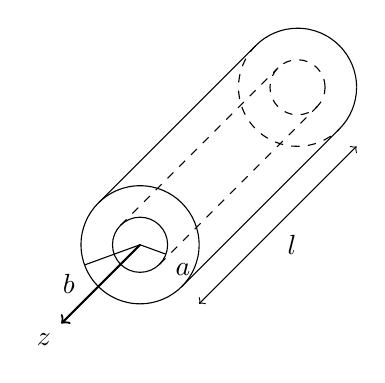
\begin{tikzpicture}
		% Achsen zeichnen
		\draw[->,thick] (0,0) -- (-1,-1) node [below left] {$z$};
		%Plot
		\draw (0,0) circle (.35);
		\draw (0,0) circle (.75);
		\draw (0,0) -- (340:.35) node [below right] {$a$};
		\draw (0,0) -- (200:.75) node[below left] {$b$};
		\draw (135:.75) --+ (2,2);
		\draw[style=dashed] (135:.35) --+ (2,2);
		\draw[style=dashed] (315:.35) --+ (2,2);
		\draw (315:.75) --+ (2,2);
		\draw[style=dashed] (2,2) circle (.35);
		\draw (2,2) +(0:.75) arc (0:135:0.75) ;
		\draw[style=dashed] (2,2)+(135:.75) arc (135:315:.75);
		\draw (2,2) +(315:.75) arc (315:360:.75);
		\draw[<-] (.75,-0.75)--(1.75,0.25) node[below right] {$l$};
		\draw[->] (1.75,0.25)--(2.75,1.25);
	\end{tikzpicture}

	\begin{tikzpicture}
		% Achsen zeichnen
		%\draw[->,thick] (0,0) -- (-1,-1) node [below left] {$z$};
		\draw[<->] (0,0)--(0,2) node[left] {$2b$} --(0,4);
		\draw[<->] (1,1.5)--(1,2) node[left] {$2a$} --(1,2.5);
		\draw (1.5,4)--(5.5,4);
		\draw (1.5,0)--(5.5,0)--(5.5,2);
		\draw[->] (1.5,2)--(7,2) node[right] {$z$};
		\draw (1.5,0)--(1.5,2);
		\draw (1.5,1) circle(.25);
		\draw[<-] (1.1,.75)--(1.1,1.25) node[below left] {$ U_0$};
		\draw (1.9,1.5) rectangle (5,2.5);
		\draw[style=dashed] (1.9,2.5)--(1.9,4.2) node[above] {$0$};
		\draw[style=dashed] (3.5,2.5)--(3.5,4.2) node[above] {$z$};
		\draw[fill=black] (1.7,0) circle(.05);
		\draw[fill=black] (1.7,2) circle(.05);
		\draw[fill=black] (5.3,0) circle(.05);
		\draw[fill=black] (5.3,2) circle(.05);
		\draw[fill=white] (5.35,0.5) rectangle (5.65,1.5);
		\node[right] at (5.75,1) {$ R$};
		\node[right] at (3,1.65) {$\kappa$};
		\node[right] at (3,-.3) {$\kappa_a \rightarrow \infty$};
		\node[right] at (3.2,.75) {$ U ( z)$};
		\draw[->] (3.2,1.3)--(3.2,0.2);
	\end{tikzpicture}
}}
		  \end{center}
		 Zur Lösung des Problems werden Maschengleichungen angesetzt:
		  	\begin{align*}
		  		\text{große Masche:}  &  & U_0  & = R_i(l)I_0 + RI_0                               \\
		  		\text{kleine Masche:} &  & U_0  & = U(z) + R_i(z)I_0                               \\
		  		\implies                   &  & U(z) & = U_0\left(1-\frac{z}{l+\kappa\pi a^2 R} \right)
		  	\end{align*}
		  Außerhalb des Leiters ist ist kein Magnetfeld vorhanden (Kompensation von Hin- und Rückstrom). Durch Anwendung von \ref{durchf} erhält man das Magnetfeld im Innenleiter ($H^i$) und im Zwischenraum zwischen den Leitern ($H^a$):
		  \begin{equation*}
		  	\vec{H} ^i = H_\varphi^i \vu{\varphi} = \frac{I_0}{2\pi a}\frac{\rho}{a} \vu{\varphi} \text{ und } \vec{H} ^a = H_\varphi^a \vu{\varphi} = \frac{I_0}{2\pi \rho} \vu{\varphi}
		  \end{equation*}
		  	Das elektrische Feld im Innenleiter hat nur eine $z$-Komponente (wegen der Stromdichte): $$\vec{E}^i=E_z^i \vec{e_z} = \frac{\vec{J}_z}{\kappa}\vec{e_z}=\frac{I_0}{\kappa\pi a^2}\vec{e_z}$$	Würde es sich bei dem Strom $I$ um einen höherfrequenten Wechselstrom handeln, dann müsste der Skineffekt ($\nearrow$\ref{skin}) beachtet werden. Weil die Stromdichte außen größer ist, haben sowohl das $E-$Feld als auch das $H-$Feld im Leiter eine andere Form. Für das elektrische Feld im Zwischenraum muss die Laplacegleichung $\Delta \phi =0$ gelöst werden, es lässt sich zeigen, dass es hier ein Skalarpotential gibt. Dafür wird diese zunächst in Zylinderkoordinaten geschrieben:
		  		$$
		  		\frac{1}{\rho}\frac{\partial}{\partial \rho}\left(\rho\frac{\partial \phi}{\partial \rho}\right) + \frac{1}{\rho^2}\frac{\partial^2 \phi}{\partial \varphi^2} + \frac{\partial^2 \phi}{\partial z^2} =0 
		  		$$
		  		Diese kann dann mit dem Separationsansatz ($\nearrow$\ref{sep}) gelöst werden. Das elektrische Feld wird dann über $\vec{E}=-\grad \phi$ errechnet. Weiterhin kann man mit \ref{tanE} die Randbedingungen $E_z^a(\rho=a) = E_z^i$ und $E_z^a(\rho=b) = 0$ gewinnen. Außerdem lässt sich eine Anfangsbedingung formulieren (siehe Skizze): $U_0=\int\limits_a^b E^a_\rho(\rho, z=0)\dd\rho$.
Schließlich ergibt das:
		  	$$
		  	E_\rho^a = \frac{U_0}{\rho \ln\frac{b}{a}}\left(1-\frac{z}{l+\kappa\pi a^2 R}\right) \quad E_z^a = \frac{U_0 \ln\frac{b}{\rho}}{\ln\frac{b}{a}}\frac{1}{l+\kappa\pi a^2 R}
		  	$$
Nun kann der komplexe Poynting Vektor aus den Feldern berechnet werden:
		  	\begin{equation*}\begin{split}
		  			\vec{\ubar{S}}^i &= \frac{1}{2} \ubar{\vec{E}}^i \times \vec{\ubar{H}}^{i\star} = -\frac{1}{2} E_z^i H_\varphi^i \vec{e_\rho}\\
		  			\vec{\ubar{S}}^a &=\frac{1}{2} \ubar{\vec{E}}^a \times \vec{\ubar{H}}^{a\star} = -\frac{1}{2} E_z^a H_\varphi^a \vec{e_\rho} + \frac{1}{2} E_\rho^a H_\varphi^{a\star} \vec{e_z}
		  	\end{split}\end{equation*}
		  Da $\vec{\ubar{S}}^i$ und $\vec{\ubar{S}}^a$ rein reell sind, wird nur Wirkleistung umgesetzt ($\omega L\ll R_i$ wurde explizit vernachlässigt!). Die radial (in $\rho$-Richtung) nach innen fließende Energie berechnet sich nach \ref{poyntint} zu:
		  	$$
		  	- 2\pi a \int\limits_0^l \vec{\ubar{S}}^i (\rho=a)\cdot\vec{e_\rho} \dd z = \frac{1}{2} R_i(l) I_0^2 
		  	$$
		  	Der Faktor $\frac{1}{2}=\frac{1}{\sqrt{2}^2}$ kommt dabei dadurch zustande, dass mit Effektivwerten gerechnet wird. Berechnet wurde damit die Verlustleistung im Innenleiter. Im Innenleiter wird also thermische Energie freigesetzt, welche aus dem Zwischenraum kommt. Dort erfolgt nämlich auch ein axialer Energietransport (in $z$-Richtung):
		  	$$
		  	\int\limits_a^b \vec{\ubar{S}}^a (\rho) \cdot\vec{e_z} 2 \pi\rho\dd\rho = \frac{1}{2} I_0 U(z)
		  	$$
		  	 Dieser Ausdruck ausgewertet bei $z=0$ ergibt die von der Quelle abgegebene Leistung. Diese ist wie erwartet:
		  	$$
		  	P = \frac{1}{2} I_0U(0) = \frac{1}{2} \frac{U_0^2}{R+R_i(l)}
		  	$$
Der Energietransport in Ausbreitungsrichtung (axial) findet nur im Zwischenraum statt, obwohl dort kein Leiter ist. Im Innenleiter und Außenleiter kommt es nur zu Verlusten.
 \section{Impulserhaltung}
 \subsection{Rolle des Impulses in der elektromagnetischen Feldtheorie}
In der Mechanik besteht eine elementare Beziehung zwischen \textbf{Impuls} \(\vec{p}^\text{ mech}\) und \textbf{Kraft} \(\vec{F} \):
\begin{equation}\label{krafimp}
	\vec{F}  = \frac{\dd}{\dd t} \vec{p}^\text{ mech}
\end{equation}
 Diese Beziehung gilt auch für den \textbf{relativistischen Impuls} (bei sehr hohen Geschwindigkeiten, im Rahmen der Speziellen Relativitätstheorie $\nearrow$\ref{SRT}) und ist somit wesentlich fundamentaler als die klassische Formulierung \(\vec{F}  = m\vec{a}\). Es gilt mit $\gamma$ als Lorentzfaktor und $m_0$ als Ruhemasse:  \begin{equation}
 	\vec{p}^\text{ mech} = \gamma m_0 \vec{v}
 	\end{equation}
 Die elektromagnetische Feldtheorie ist eine relativistische Theorie, weshalb es sinnvoll ist den Impuls zu betrachten.
 \subsection{Kraftdichte}
  Zudem kann in der elektromagnetischen Feldtheorie die Lorentzkraft ($\nearrow$\ref{lorentz}) herangezogen werden. In simplen Situationen (bspw. wenn sich eine Punktladung frei durch ein homogenes Magnetfeld bewegt) ist das zweckmäßig. Für kompliziertere praktische Berechnungen (z.B. elektrische Antriebe) wird das unhandlich, weshalb \textbf{Formulierung nur mit Feldern} angebrachter ist (letztlich ist es nur eine \enquote{Umschreibung} der Lorentzkraft).\\
 Die lokale \textbf{Kraftdichte} \(\vec{f}\) in Abhängigkeit von der \textbf{Impulsdichte} \(\vec{p}_\text{V}^\text{ mech}\) ist durch Ersetzung der Kraft und des Impulses durch die jeweilige Dichte in \ref{krafimp} gegeben:
		        \begin{equation}
			        \vec{f}= \frac{\dd}{\dd t} \vec{p}_\text{V}^\text{ mech} \quad \quad \vec{F} =\iiint\limits_V \vec{f}\, \dd V
		        \end{equation}
Mit \ref{lorentz} und \ref{jrhov} lässt sich für die Kraftdichte schreiben (Ladung $\leftrightarrow$ Ladungsdichte):
		        \begin{equation}\label{kraftdicht}
			        \vec{f}= \frac{\dd}{\dd t}\vec{p}_\text{V}^\text{mech} =\rho_\text{V} (\vec{E} + \vec{v} \times \vec{B} ) = \textcolor{green}{\rho_\text{V}} \vec{E} + \textcolor{red}{\vec{J}} \times \vec{B}
		        \end{equation}
		   Durch Einsetzen der Maxwell-Gleichungen ($\nearrow$\ref{ind},\ref{quellf},\ref{durchf},\ref{gauss}) sowie anwenden einer Produktregel folgt:
		        \begin{align}
			        \vec{f} & =  \vec{E}\, \textcolor{green}{\div \vec{D} } + \textcolor{red}{(\rot \vec{H} -\frac{\partial \vec{D} }{\partial t})} \times \vec{B}   \nonumber                                                                                                                \\
			                & = \vec{E}\, \div \vec{D}  + (\rot \vec{H} ) \times \vec{B}  - \frac{\partial \vec{D} }{\partial t}  \times \vec{B}   \nonumber                                                                                                                                  \\
			                & = \vec{E}\, \div \vec{D}  + (\rot \vec{H} ) \times \vec{B}  - \left[ \frac{\dd }{\dd t}(\vec{D}  \times \vec{B} ) \textcolor{red}{-} \vec{D}  \times \textcolor{red}{\frac{\partial \vec{B} }{\partial t}} \right]  \nonumber                             \\
			                & = \vec{E}\, \div \vec{D}  + \underbrace{(\rot \vec{H} ) \times \vec{B}}_{\vec{a}\times\vec{b}=-\vec{b}\times\vec{a}}  - \left[ \frac{\dd }{\dd t}(\vec{D}  \times \vec{B} ) \textcolor{red}{+} \vec{D}  \times \textcolor{red}{\rot \vec{E}}\nonumber \right]      \end{align}
			                Umordnen liefert:
			                \begin{align}
			        \Aboxed{\vec{f} & = \left[ \vec{E}\, \div \vec{D}  - \vec{D}  \times \rot \vec{E}\right] + \left[-\vec{B} \times ( \rot \vec{H} )\right] - \frac{\dd }{\dd t}(\vec{D}  \times \vec{B} )} \quad \text{ alle Materialien}\\
			                & = \left[ \vec{E}\, \div \vec{D}  - \vec{D}  \times \rot \vec{E}\right] + \left[\vec{H} \,\textcolor{red}{\underbrace{\div \vec{B}}_{=0, \text{für Symmetrie} }}-\vec{B} \times \rot \vec{H} \right] - \frac{\dd }{\dd t}(\vec{D}  \times \vec{B} )\nonumber\\
			       \Aboxed{\vec{f}& = \varepsilon\left[ \vec{E}\, \div \vec{E} - \vec{E} \times \rot \vec{E}\right] + \frac{1}{\mu}\left[\vec{B} \,\div \vec{B} -\vec{B} \times \rot \vec{B} \right] - \varepsilon\frac{\dd }{\dd t}(\vec{E} \times \vec{B} ) } \quad \text{ hli}
		        \end{align}
	Mit \ref{gradab} folgt:	   
		        \begin{equation*}\begin{split}
				         - \vec{E} \times \rot \vec{E} &= (\vec{E}\cdot\grad )\vec{E} - \frac{1}{2}\grad |\vec{E}|^2\quad \text{ für }\vec{B} \text{ analog}
			        \end{split}\end{equation*}
		   Damit ist die \textbf{Kraftdichte in homogenen, lineare, isotropen Medien}:
		        \begin{equation}
		        	\boxed{
			        \begin{split}
				        \vec{f}=  \varepsilon\left[ \vec{E}\, \div \vec{E} +(\vec{E}\cdot\grad )\vec{E}\right] + \frac{1}{\mu}\left[\vec{B} \,\div \vec{B}  + (\vec{B} \cdot\grad )\vec{B} \right] \\-\grad \underbrace{\left[ \frac{1}{2}\varepsilon|\vec{E}|^2 +\frac{1}{2\mu} |\vec{B} |^2  \right]}_{w_\text{em}}- \underbrace{\varepsilon\frac{\dd }{\dd t}(\vec{E} \times \vec{B} )}_{\varepsilon\mu\frac{\dd }{\dd t} \vec{S}}
			        \end{split}}
		        \end{equation}
  \subsection{Maxwellscher Spannungstensor}\label{spanten}
  \subsubsection{Definition}
         Um die Kraftdichte einfacher schreiben zu können, wird der \textbf{Maxwellsche Spannungstensor} \(\mathbf{T}\) eingeführt. Dieser ist ein dreidimensionaler Tensor 2. Stufe (\enquote{\(3 \times 3\)-Matrix}):
              \begin{equation}\label{maxkofrei}
	              \mathbf{T} = \left(T_{ij}\right) \text{ mit } \boxed{T_{ij} = \varepsilon\left[ E_iE_j-\frac{1}{2}\delta_{ij} |\vec{E}|^2\right] + \frac{1}{\mu} \left[B_iB_j-\frac{1}{2}\delta_{ij} |\vec{B} |^2\right] } 
              \end{equation}
         Diese Darstellung ist zunächst noch Korrdinatenfrei ($\nearrow$\ref{maxkofreiaus}). Explizit lässt sich in kartesischen Koordinaten schreiben:
              \begin{equation}
	              \begin{split}
		              \mathbf{T} =
		              \begin{pmatrix}
			              \varepsilon E_xE_x + \frac{1}{\mu}B_xB_x & \varepsilon E_xE_y + \frac{1}{\mu}B_xB_y & \varepsilon E_xE_z + \frac{1}{\mu}B_xB_z \\
			              \varepsilon E_yE_x + \frac{1}{\mu}B_yB_x & \varepsilon E_yE_y + \frac{1}{\mu}B_yB_y & \varepsilon E_yE_z + \frac{1}{\mu}B_yB_z \\
			              \varepsilon E_zE_x + \frac{1}{\mu}B_zB_x & \varepsilon E_zE_y + \frac{1}{\mu}B_zB_y & \varepsilon E_zE_z + \frac{1}{\mu}B_zB_z
		              \end{pmatrix}
		              \\ -\underbrace{\frac{1}{2}\left(\varepsilon |\vec{E}|^2 + \frac{1}{\mu}|\vec{B} |^2\right)}_{w_\text{em}}
		              \begin{pmatrix}
			              1 & 0 & 0 \\
			              0 & 1 & 0 \\
			              0 & 0 & 1
		              \end{pmatrix}
	              \end{split}
              \end{equation}
 An der expliziten Formulierung sieht man, dass der Tensor symmetrisch ist. In \(T_{ij}\) steht das $i$ (bzw. $j$, egal wegen Symmetrie) für die \textbf{Wirkrichtung} der Kraft pro Flächeneinheit (Druck). Diese Kraft wirkt auf das Flächenelement mit Normale \(\vu{j}\) (bzw. $\vu{i}$), weshalb man diese Richtung auch als \textbf{Normalenrichtung} bezeichnet.  Die Komponenten, für die \(i=j\) gilt (\(T_{ii}\)) heißen \textbf{Normalspannungskomponenten}, bei denen Normalen- und Wirkrichtung gleich sind. Die Komponenten mit \( i \ne j \) heißen \textbf{Scherspannungskomponenten}, bei den Normalen- und Wirkrichtung unterschiedlich sind. Die folgende Abbildung verbildlicht einen Spannungstensor an einem Volumenelement $\dd V$. In einem größeren Volumen sind anschaulich viele solcher Volumenelmente zusammengesetzt. Zur Berechnung der resultierenden Kraft auf das gesamte Volumen werden letztlich alle Kraftkomponenten über die Oberfläche kumuliert. Gibt es eine resultierende Kraft muss sich das Volumen bewegen (oder mechanisch befestigt sein $\to$ Kräftegleichgewicht). Anschauung (\href{https://tex.stackexchange.com/questions/553898/how-to-draw-a-cube-with-coordinate-systems-in-tikz}{Bildquelle}):
 \begin{center}
 	\resizebox{!}{.3\textwidth}{ \begin{tikzpicture}[%
	3d view = {15}{15}
	]
	
	\draw[-{Latex[scale = 0.7]}] (-4, -4, 0) -- (-3, -4, 0)
	node[below] {$x_1$};
	\draw[-{Latex[scale = 0.7]}] (-4, -4, 0) -- (-4, -3, 0)
	node[right] {$x_2$};
	\draw[-{Latex[scale = 0.7]}] (-4, -4, 0) -- (-4, -4, 1)
	node[above] {$x_3$};
	
	\begin{scope}[canvas is xz plane at y = -2]
		
		\draw[
		fill = lightgray
		] (-2, -2) rectangle (2, 2);
		
		\draw[-Latex] (-1.75, 0) -- (1.75, 0)
		node[below left] {$T_{12}$};
		\draw[-Latex] (0, -1.75) -- (0, 1.75)
		node[below left] {$T_{32}$};
		
	\end{scope}     
	
	\draw[Latex-] (0, -2, 0) -- (0, -3.5, 0)
	node[left] {$T_{22}$};
	
	\begin{scope}[canvas is yz plane at x = 2]
		
		\draw[
		fill = lightgray
		] (-2, -2) rectangle (2, 2);
		
		\draw[-Latex] (1.75, 0) -- (-1.75, 0)
		node[below right] {$T_{21}$};
		\draw[-Latex] (0, -1.75) -- (0, 1.75)
		node[below right] {$T_{31}$};
		
	\end{scope} 
	
	\draw[Latex-] (2, 0, 0) -- (3.5, 0, 0)
	node[right] {$T_{11}$};
	
	\begin{scope}[canvas is xy plane at z = 2]
		
		\draw[
		fill = lightgray
		] (-2, -2) rectangle (2, 2);
		
		\draw[-Latex] (-1.75, 0) -- (1.75, 0)
		node[above]{$T_{13}$};
		\draw[-Latex] (0, 1.75) -- (0, -1.75)
		node[above left]{$T_{23}$};
		
	\end{scope} 
	
	\draw[Latex-] (0, 0, 2) -- (0, 0, 3.5)
	node[above] {$T_{33}$};
	
\end{tikzpicture}}
 \end{center}
Wie mit dem Spannungstensor gerechnet werden kann, insbesondere wie das Flächenintegral behandelt wird, ist in \ref{dyad} aufgegriffen. In der relativistisch kovarianten Formulierung der Elektrodynamik wird mit dem \href{https://en.wikipedia.org/wiki/Covariant_formulation_of_classical_electromagnetism#Electromagnetic_stress%E2%80%93energy_tensor}{Energie-Impuls-Tensor} (\enquote{$4\times 4$}, wegen Vierervektoren) gearbeitet, welcher als Komponenten die des Maxwellschen Spannungstensors enthält.
  \subsubsection{Zusammenhang mit Kraftdichte}
  Die Divergenz eines Tensors 2. Stufe ist ein Tensor 1. Stufe. Die \(j\)-te Komponente der Divergenz von \(\mathbf{T}\) ist definiert als:
		        \begin{equation}\begin{split}
				        (\div \mathbf{T})_j &= \sum_{i=1}^3 \frac{\partial}{\partial x_i} T_{ij} = \partial_i T_{ij} \\
				        &= \sum_{i=1}^3 \left\{ \varepsilon\left( \frac{\partial E_i}{\partial x_i} E_j + E_i\frac{\partial E_j}{\partial x_i} \right) +
				        \frac{1}{\mu}\left( \frac{\partial B_i}{\partial x_i} B_j + B_i\frac{\partial B_j}{\partial x_i} \right)
				        \right\} - \left(\frac{\varepsilon}{2}\frac{\partial |\vec{E}|^2}{\partial x_j} + \frac{1}{2\mu}\frac{\partial |\vec{B} |^2}{\partial x_j}\right)\\
				        &=\varepsilon\left[E_j \div \vec{E} + (\vec{E}\cdot\grad )E_j - \frac{1}{2}\grad _j |\vec{E}|^2 \right] +\\
				        &\qquad \frac{1}{\mu}\left[B_j \div \vec{B}  + (\vec{B} \cdot\grad )B_j - \frac{1}{2}\grad _j |\vec{B} |^2 \right]
			        \end{split}\end{equation}
		   Dies ist gerade die \(j\)-te Komponente der ersten drei Terme der Kraftdichte. Somit:
		        \begin{equation}\label{kraftdmax}
			        \boxed{\vec{f}= \div \mathbf{T} - \varepsilon\frac{\dd}{\dd t}\left( \vec{E} \times \vec{B} \right)
				        = \div \mathbf{T} - \varepsilon\mu\frac{\dd}{\dd t}\left( \vec{E} \times \vec{H} \right)
				        = \div \mathbf{T} - \varepsilon\mu\frac{\dd \vec{S}}{\dd t}}
		        \end{equation}
		   Die Gesamtkraft (die wirkende Kraft auf das Probevolumen $V$, bspw. eine Kondensatorplatte) ist somit:
		        \begin{equation}
			        \boxed{\vec{F}  = \oiint\limits_{O(V)} \mathbf{T} \cdot \dd\vec{A} - \varepsilon\mu\frac{\dd}{\dd t} \iiint\limits_V \vec{S} \dd V}
		        \end{equation}
	  Das \textbf{Oberflächenintegral} liefert einen Beitrag zur Gesamtkraft, der nur auf die Oberläche des betrachteten Volumens wirkt. Das \textbf{Volumenintegral} verschwindet im stationären Fall. Dann wird die Gesamtkraft nur über die Oberfläche bestimmt. In Analogie zur Mechanik ($\nearrow$\ref{krafimp}), in der die zeitliche Ableitung eines Impulses eine Kraft ist, kann man den \textbf{elektromagnetischen Impuls} bzw. eine entsprechende \textbf{Impulsdichte} definieren:
		        \begin{align}
			       \Aboxed{ \vec{p}^\text{ em}   & = \iiint\limits_V \varepsilon\mu\vec{S} \dd V }\\
			        \Aboxed{\vec{p}^\text{ em}_V & = \varepsilon\mu\vec{S}} \label{impdicht}
		        \end{align}
Die hier zu Tage tretende enge Verbindung von Energie (Poynting-Vektor) und Impuls sieht man auch in der kovarianten Formulierung der Elektrodynamik deutlich. Man arbeitet mit dem \href{https://en.wikipedia.org/wiki/Covariant_formulation_of_classical_electromagnetism#Electromagnetic_stress%E2%80%93energy_tensor}{Energie-Impuls-Tensor}. 
  \subsection{Formulierung der Impulserhaltung}
		  Unter Beachtung von \ref{kraftdicht} kann man für \ref{kraftdmax} nun schreiben:
		        \begin{align}
			        \vec{f}= \frac{\dd }{\dd t}\vec{p}^\text{ mech}_V                              & = \div \mathbf{T} - \frac{\dd }{\dd t}\left( \varepsilon\mu\vec{S}\right) = \div \mathbf{T} - \frac{\dd }{\dd t}\vec{p}^\text{ em}_V \nonumber \\
			        \frac{\dd }{\dd t}\left(\vec{p}^\text{ mech}_V +  \varepsilon\mu\vec{S}\right) & =\div \mathbf{T}                                                                                                                     \nonumber\\
			        \Aboxed{\frac{\dd }{\dd t}\left(\vec{p}^\text{ mech}_V + \vec{p}^\text{ em}_V\right)   & =\div \mathbf{T}}
		        \end{align}
		   Die Volumenintegration dieser \textbf{lokalen Impulsbilanz} liefert die \textbf{integrale Impulsbilanz}:
		        \begin{equation}
			        \boxed{\frac{\dd }{\dd t} \iiint\limits_V \left(\vec{p}^\text{ mech}_V + \vec{p}^\text{ em}_V\right)\dd V = \oiint\limits_{O(V)}\mathbf{T} \cdot \dd \vec{A}}
		        \end{equation}
\section{Verallgemeinerte Betrachtungen zur Eichung}\label{geneich}
\subsection{Potentiale} 
In diesem Abschnitt sollen die mikroskopischen Maxwellgeichungen \textbf{im Vakuum} betrachtet werden ($\nearrow$\ref{mikrosmax}). Die Felder und Quellen sind stetig differenzierbare Funktionen des Ortes $\vec{{r}}$ und der Zeit ${t}$. Über die zeitlichen Ableitungen der Feldgrößen $\vec{E}$ und $\vec{B}$ sind die Gleichungen verkoppelt.\\
Bei der Lösung der MGl ist es manchmal hilfreich, das elektrische \textbf{Skalarpotential} $\phi$ und das magnetische \textbf{Vektorpotential} $\vec{A}$ einzuführen. Rotationsfreie Felder sind als Gradient darstellbar und divergenzfreie Felder als Rotation ($\nearrow$\ref{poin}).
 \begin{align}
	\div \vec{B} & = 0                                     & \Rightarrow \quad    & \boxed{\vec{B} =\rot  \vec{A}}                                        \label{potadef}   \\
	\rot \vec{E} & = -\frac{\partial \vec{B} }{\partial t} & \Rightarrow  \quad   & \rot \vec{E} = -\rot \frac{\partial  \vec{A}}{\partial t}              \nonumber  \\
	&                                         & \Leftrightarrow\quad & \rot \left(\vec{E}+\frac{\partial  \vec{A}}{\partial t}\right) = \vec{0} \nonumber\\
	&                                         & \Rightarrow  \quad   & \vec{E}+\frac{\partial  \vec{A}}{\partial t} = -\grad \phi      \nonumber         \\
	&                                         & \Rightarrow \quad    & \boxed{\vec{E}=-\grad \phi -\frac{\partial  \vec{A}}{\partial t}} \label{potsdef}
\end{align}
Mit den so definierten Beziehung zwischen den Feldern und den Potentialen ist garantiert, dass die homogenen Maxwellgleichungen ($\nearrow$ \ref{ind},\ref{quellf}) automatisch erfüllt werden.
\begin{align}
	\div\vec{B} & =\div\rot \vec{{A}} \equiv 0 \quad \text { für beliebiges } \vec{{A}} \label{auterf1}\\
	\rot \vec{E}+\frac{\partial\vec{B}}{\partial {t}} & =\rot\left(-\grad \phi-\frac{\partial \vec{{A}}}{\partial {t}}\right)+\frac{\partial}{\partial {t}}(\rot \vec{{A}}) \nonumber \\
	& =-\rot\left(\frac{\partial \vec{{A}}}{\partial {t}}\right)+\frac{\partial}{\partial {t}}(\rot \vec{{A}}) \equiv \vec{0} \quad \text { für beliebiges } \phi \text { und } \vec{{A}} \label{auterf2}
\end{align}
Das Einsetzen der Gleichungen \ref{potadef} und \ref{potsdef} in die inhomogenen Maxwellgleichungen ($\nearrow$\ref{durchf}\ref{gauss}) ergibt unter Nutzung der Identität \ref{rotrot} die Bestimmungsgleichungen für die Potentiale (hier im Vakuum, für homogen linear, isotrop ersetze $\mu_{0}\leftrightarrow\mu$,$\varepsilon_{0}\leftrightarrow\varepsilon$):        
\begin{align}
	\div\left(-\grad \phi-\frac{\partial \vec{{A}}}{\partial {t}}\right)=\frac{\rho_\text{V}}{\varepsilon_{0}} \implies \boxed{ \Delta \phi+\div \frac{\partial \vec{{A}}}{\partial {t}}=-\frac{\rho_\text{V}}{\varepsilon_{0}} } \label{bestphi}\\
	\rot(\rot \vec{{A}})-\varepsilon_{0} \mu_{0} \frac{\partial}{\partial {t}}\left(-\grad \phi-\frac{\partial \vec{{A}}}{\partial {t}}\right)=\mu_{0} \vec{{J}} \nonumber\\
	\implies \Aboxed{ \Delta \vec{{A}}-\varepsilon_{0} \mu_{0} \frac{\partial^{2} \vec{{A}}}{\partial {t}^{2}}=-\mu_{0} \vec{{J}}+\grad\left(\varepsilon_{0} \mu_{0} \frac{\partial \phi}{\partial {t}}+\div \vec{{A}}\right) } \label{besta}
\end{align}
Störend ist hier die Verkopplung ($\phi,A$ kommen in einer Gleichung vor) der beiden Gleichungen. Dies führt zur Eichung.
\subsection{Eichtransformation}
Zunächst soll eine bezüglich $\vec{{r}}$ und ${t}$ zweifach stetig differenzierbare Funktion $\psi=\psi(\vec{r}, {t})$ betrachtet werden. Mit Hilfe dieser Funktion $\psi$ wird die folgende \textbf{Eichtransformation} definiert:
\begin{equation}\label{geneichtrans}
	\boxed{\phi^{\prime}=\phi-\frac{\partial \psi}{\partial {t}}} \quad\quad\quad \boxed{ \vec{{A}}^{\prime}=\vec{{A}}+\grad \psi }
\end{equation}
Die Transformation \ref{geneichtrans} ist sinnvoll, weil so eine \textbf{Eichinvarianz} gilt, also die Felder gleich bleiben. Die Felder sind physikalische Größen und keine Hilfsgrößen, sie dürfen durch den Lösungsweg nicht geändert werden. Es gilt:
\begin{align*}
	\vec{B}^{\prime}&=\rot \vec{{A}}^{\prime}=\rot(\vec{{A}}+\grad \psi)=\rot \vec{{A}}+\underbrace{\rot \grad \psi}_{\equiv \vec{0}}=\vec{{B}}  \\
	\vec{E}^{\prime}&=-\grad \phi^{\prime}-\frac{\partial \vec{{A}}^{\prime}}{\partial {t}}=-\grad\left(\phi-\frac{\partial \psi}{\partial {t}}\right)-\frac{\partial}{\partial {t}}(\vec{{A}}+\grad \psi) \\
	&=-\grad \phi+\grad \frac{\partial \psi}{\partial {t}}-\frac{\partial \vec{{A}}}{\partial {t}}-\frac{\partial}{\partial {t}} \grad \psi \\
	&=-\grad \phi-\frac{\partial \vec{{A}}}{\partial {t}}=\vec{E}
\end{align*}
Die Bestimmungsgleichungen für die in \ref{potadef} und \ref{potsdef} definierten Potentiale sind in \ref{bestphi} und \ref{besta} gegeben. Diese sind in dieser Form kompliziert und sollen vereinfacht werden. Addiert man also wie in \ref{geneichtrans} $\psi$-enthaltende Terme zu den Potentialen, bleiben die eigentlichen physikalischen Größen gleich. Man kann somit die Potentiale manipulieren, sodass sie spezielle Bedingungen, die \textbf{Eichbedingungen}($\nearrow$\ref{coulbdg}, \ref{lorenzbdg}, \ref{vbdg}), erfüllen, ohne dabei die eigentlichen Felder zu verändern (\textbf{Eichfreiheit}). Wenn man für diese Bedingungen allgemein die Existenz von $\psi$ zeigen kann, also beweisbar ist, dass man immer ein $\psi$ finden kann, sodass die Eichbedingungen erfüllt sind, ist das konkrete Aussehen von $\psi$ nicht mehr von Interesse. Man kann ohne Weiteres die Vereinfachungen \ref{bestskalcoul}, \ref{bestvekcoul}, \ref{bestskalarpotlor}, \ref{bestvekpotlor}, \ref{bestskav} und \ref{bestvekv} der Bestimmungsgleichungen nutzen. Die Lösungen der vereinfachten Gleichungen sind in \ref{skalarpotcoul}, \ref{vekpotcoul}, \ref{skalarpotlor}, \ref{vekpotlor}, \ref{skalarpotv} und \ref{vekpotv} gegeben. Mit \ref{potadef} und \ref{potsdef} lassen sich dann die Felder berechnen.
\subsection{Divergenz des Vektorpotentials}
\subsubsection{Einfacher Fall}
% PLENUM : warum kann man $\div \vec{{A}}=\alpha(\vec{{r}}, {t})\neq f(\phi)$ annehmen??? Ringschluss???
In den allgemeinen Bestimmungsgleichungen \ref{bestphi} und \ref{besta} spielt $\div \vec{{A}}$ eine wichtige Rolle. Sei nun $\div \vec{{A}}=\alpha(\vec{{r}}, {t})\neq f(\phi)$ die tatsächliche Divergenz des Vektorpotentials $\vec{{A}}$. Es stellt sich dann die Frage, ob es für ein beliebiges $\beta(\vec{r}, t)$ eine durch $\psi$ induzierte Eichtransformation gibt, so dass $\div \vec{{A}}^{\prime}=\beta(\vec{{r}}, {t})$ ist. Man rechnet:
$$
\begin{aligned}
	 \div \vec{{A}}^{\prime}&=\div(\vec{{A}}+\grad \psi)=\div \vec{{A}}+\Delta \psi \\
	& =\alpha +\Delta \psi  \stackrel{!}{=} \beta \\
	 \Rightarrow \Delta \psi&=\beta-\alpha
\end{aligned}
$$
Diese Poisson-Gleichung für $\psi$ ist immer (und für jeden Zeitpunkt) lösbar. Die Lösung ist aber nicht eindeutig, da jede beliebige Lösung der homogenen Gleichung (Laplace-Gleichung) addiert werden kann. Alle möglichen $\psi$ nennt man \textbf{Eichklasse}. Die \textbf{Divergenz} des Vektorpotentials $\div \vec{A}$ kann in diesem Fall auf \textbf{beliebige Werte} gesetzt werden. Eine Anwendung dieses einfachen Falls ist die Coulomb-Eichung ($\nearrow$\ref{couleich}).
\subsubsection{Allgemeiner Fall}
Normalerweise kann die Divergenz des Vektorpotentials auf beliebige Werte gesetzt werden. Wenn die Divergenz des Vektorpotentials auch eine Funktion des Skalarpotentials sein soll, wie bei der Lorenz- und $v$-Eichung ($\nearrow$\ref{lorenzeich},\ref{veich}), muss man etwas anders vorgehen. Sei nun $\div \vec{A}=f(\vec{r}, t, \phi)$. Man rechnet:
\begin{align*}
	 \div \vec{{A}}^{\prime}=\div(\vec{{A}}+\grad \psi)=\div \vec{{A}}+\Delta \psi &\stackrel{!}{=} {f}\left(\vec{{r}}, {t}, \phi^{\prime}\right) \\
	&={f}\left(\vec{{r}}, {t}, \phi-\frac{\partial \psi}{\partial {t}}\right) 
\end{align*}
Dies ist im Allgemeinen keine Poisson-Gleichung mehr. Die Bestimmungsgleichung ist erst bekannt, wenn eine konkrete Abhängigkeit von $\phi$ gefordert wird. Dann muss die Existenz von $\psi$ gezeigt werden.
\subsection{Coulomb-Eichung}\label{couleich}
Unter Coulomb-Eichung versteht man eine Eichtransformation induziert durch $\psi_{{C}}$, so dass für das transformiere Vektorpotential $\vec{{A}}_{{C}}$ gilt:
\begin{equation}\label{coulbdg}
	\boxed{\div \vec{A}_{C}=0 }
\end{equation}
Die allgemeinen Bestimmungsgleichungen \ref{bestphi} und \ref{besta} der Potentiale vereinfachen sich dann zu:
\begin{align}\label{bestskalcoul}
	\Aboxed{\Delta \phi_{{C}}&=-\frac{\rho_\text{V}}{\varepsilon_{0}}} \\
	 \Aboxed{\Delta \vec{{A}}_{{C}}-\varepsilon_{0} \mu_{0} \frac{\partial^{2} \vec{{A}}_{{C}}}{\partial {t}^{2}}&=-\mu_{0} \vec{{J}}+\varepsilon_{0} \mu_{0} \grad \frac{\partial \phi_{{C}}}{\partial {t}}}\label{bestvekcoul}
\end{align}
Die Lösung für das Skalarpotential $\phi_{{C}}$ ergibt sich unmittelbar aus der Kenntnis der Greenschen Funktion ($\nearrow$ \ref{greenLaplace}) des Laplace Operators zu (beachte, dass sich hier auf den Freiraum beschränkt wurde):
\begin{equation}\label{skalarpotcoul}
	\boxed{\phi_{{C}}(\vec{{r}}, {t})=\frac{1}{4 \pi \varepsilon_{0}} \iiint \frac{\rho_\text{V}\left(\vec{{r}}^{\prime}, {t}\right)}{\left|\vec{{r}}-\vec{{r}}^{\prime}\right|} \dd^3 {r}^{\prime}} 
\end{equation}
 Will man eine explizite Lösung für das Vektorpotential $\vec{A}_{C}$ in Coulomb-Eichung angeben, muss man in der Bestimmungsgleichung \ref{bestvekcoul} das Skalarpotential $\phi_{{C}}$ eliminieren.  Nach dem Helmholtz-Theorem ($\nearrow$\ref{helmholtz}) ist eine Zerlegung eines Vektorfeldes $\vec{f}(\vec{r}, t)$ in einen longitudinalen, rotationsfreien Anteil $\vec{f}_{l}(\vec{r}, t)=\vec{\alpha}(\vec{r}, t)$ und einen transversalen, divergenzfreien Anteil $\vec{{f}}_{{t}}(\vec{{r}}, {t})=\vec{\beta}(\vec{{r}}, {t})$ möglich, also:
\begin{equation}\label{coulzerl1}
\vec{{f}}(\vec{{r}}, {t})=\vec{\alpha}(\vec{{r}}, {t})+\vec{\beta}(\vec{{r}}, {t}) \text { mit }\left\{\begin{array}{l}
	\rot \vec{\alpha}=0 \implies \vec{\alpha}=-\grad {a}  \\
	\div \vec{\beta}=0 \implies \vec{\beta}=\rot \vec{{b}}
\end{array}\right.
\end{equation}
Die Felder $a$ und $\vec{b}$ werden unter Kenntnis der Greenschen Funktion des Laplace-Operators ($\nearrow$\ref{greenLaplace}) folgendermaßen berechnet:
\begin{equation}\label{coulzerl2}
	{a}=\frac{1}{4 \pi} \iiint \frac{\div_{{r}^{\prime}} \vec{{f}}\left(\vec{r}^{\prime}, {t}\right)}{\left|\vec{{r}}-\vec{{r}}^{\prime}\right|} \dd^3 {r}^{\prime}, \quad\quad\quad \vec{{b}}=\frac{1}{4 \pi} \iiint \frac{\rot_{{r}^{\prime}} \vec{{f}}\left(\vec{r}^{\prime}, {t}\right)}{\left|\vec{{r}}-\vec{{r}}^{\prime}\right|} \dd^3 {r}^{\prime} 
\end{equation}
Die Zerlegung \ref{coulzerl1} mit den Beziehungen \ref{coulzerl2} kann nun auf die Stromdichte $\vec{J}$ angewendet werden:
\begin{equation}\label{jzerl}
\vec{J}=\vec{J}_{l}+\vec{J}_{t} \text { mit }\left\{\begin{array}{l}
	\vec{J}_{l}(\vec{r}, t)=-\grad\left(\frac{1}{4 \pi} \iiint \frac{\div_{r^{\prime}} \vec{J}\left(\vec{r}^{\prime}, t\right)}{\left|\vec{r}-\vec{r}^{\prime}\right|} d^{3} r^{\prime}\right)  \\
	\vec{J}_{t}(\vec{r}, t)=\rot\left(\frac{1}{4 \pi} \iiint \frac{\rot_{r^{\prime}} \vec{J}\left(\vec{r}^{\prime}, t\right)}{\left|\vec{r}-\vec{r}^{\prime}\right|} d^{3} r^{\prime}\right)
\end{array}\right.
\end{equation}
Für Probleme mit $\div \vec{J}=0$ ist $\vec{J}_{t}=\vec{J}$. Für die Zeitableitung von \ref{skalarpotcoul} folgt dann mit Hilfe der Kontinuitätsgleichung \ref{kont}:
\begin{equation}\label{skalarabl}
	\frac{\partial \phi_{{C}}(\vec{{r}}, {t})}{\partial {t}}=\frac{1}{4 \pi \varepsilon_{0}} \iiint \frac{\frac{\partial \rho_\text{V}\left(\vec{{r}}^{\prime}, {t}\right)}{\partial {t}}}{\left|\vec{{r}}-\vec{{r}}^{\prime}\right|} \dd^3 {r}^{\prime}=-\frac{1}{4 \pi \varepsilon_{0}} \iiint \frac{\div_{{r}^{\prime}} \vec{{J}}\left(\vec{{r}}^{\prime}, {t}\right)}{\left|\vec{{r}}-\vec{{r}}^{\prime}\right|} \dd^3 {r}^{\prime} 
\end{equation}
Der Vergleich der longitudinalen Stromdichte in \ref{jzerl} mit der Zeitableitung des Skalarpotentials in Gleichung \ref{skalarabl} liefert schließlich einen Ausdruck für den Gradienten der Zeitableitung des Skalarpotentials:
\begin{equation}
	\grad \frac{\partial \phi_{{C}}(\vec{{r}}, {t})}{\partial {t}}=\frac{1}{\varepsilon_{0}} \vec{{J}}_{l}(\vec{{r}}, {t}) 
\end{equation}
Die Bestimmungsgleichung des Vektorpotentials in Coulombeichung aus \ref{bestvekcoul}
wird damit entkoppelt und stellt sich als Wellengleichung dar, wobei die rechte Seite durch den transversalen Anteil der Stromdichte bestimmt ist:
\begin{equation}
	\Delta \vec{{A}}_{{C}}-\varepsilon_{0} \mu_{0} \frac{\partial^{2} \vec{{A}}_{{C}}}{\partial {t}^{2}}=-\mu_{0} \vec{{J}}+\varepsilon_{0} \mu_{0} \grad \frac{\partial \phi_{{C}}}{\partial {t}}=-\mu_{0}\left(\vec{{J}}-\vec{{J}}_{l}\right)=-\mu_{0} \vec{{J}}_{{t}} 
\end{equation}
 Die Lösung dieser Wellengleichung ist das \textbf{retardierte Vektorpotential} und folgt mit der Greenschen Funktion des Wellenoperators ($\nearrow$\ref{greenWell}):
\begin{equation}\label{vekpotcoul}
	\boxed{\vec{{A}}_{{C}}(\vec{{r}}, {t})=\frac{\mu_{0}}{4 \pi} \iiint \frac{\vec{{J}}_{{t}}\left(\vec{{r}}^{\prime}, {t}_{\text{ret}}\right)}{\left|\vec{{r}}-\vec{{r}}^{\prime}\right|} \dd^3 {r}^{\prime}} \quad\text { mit }\quad {t}_{\text{ret}}={t}-\sqrt{\varepsilon_{0} \mu_{0}}\left|\vec{{r}}-\vec{{r}}^{\prime}\right|={t}-\frac{\left|\vec{{r}}-\vec{{r}}^{\prime}\right|}{{c}} 
\end{equation}
Das Vektorpotential in Coulomb-Eichung ist retardiert mit der Geschwindigkeit $c$ und damit \textbf{kausal}. Im Gegensatz dazu ist das Skalarpotential in Coulomb-Eichung instantan und damit \textbf{nicht kausal}. Die Kausalität der Felder wird über das Vektorpotential sichergestellt.
\subsection{Lorenz-Eichung}\label{lorenzeich}
Note: Dieser Lorenz hat nichts mit dem Lorentz von \ref{lorentz} zu tun.\\
Allgemein gelten die Gleichungen \ref{bestphi} und \ref{besta} als Bestimmungsgleichungen für die Potentiale. Die Divergenz des Vektorpotentials kann beliebig gesetzt werden, in der  Lorenz-Eichung setzt man (obwohl die Existenz von $\psi$ noch gezeigt werden muss):
\begin{equation}\label{lorenzbdg}
	\boxed{\div \vec{{A}}_{{L}}=-\varepsilon_{0} \mu_{0} \frac{\partial \phi_{{L}}}{\partial {t}} }
\end{equation}
Damit nehmen die Bestimmungsgleichungen jeweils sofort die Form von Wellengleichungen an:
\begin{align}
	\Aboxed{\Delta \phi_{{L}}-\varepsilon_{0} \mu_{0} \frac{\partial^{2} \phi_{{L}}}{\partial {t}^{2}} & =-\frac{\rho_\text{V}}{\varepsilon_{0}}} \label{bestskalarpotlor}\\
	\Aboxed{\Delta \vec{{A}}_{{L}}-\varepsilon_{0} \mu_{0} \frac{\partial^{2} \vec{{A}}_{{L}}}{\partial {t}^{2}} & =-\mu_{0} \vec{{J}}}\label{bestvekpotlor}
\end{align}
erzemwell
Mit der Greenschen Funktion ($\nearrow$\ref{greenWell}) des Wellenoperators folgen sofort die retardierten (kausalen) Lösungen mit $t_{\text{ret}}={t}-\sqrt{\varepsilon_{0} \mu_{0}}\left|\vec{{r}}-\vec{{r}}^{\prime}\right|={t}-\frac{\left|\vec{{r}}-\vec{{r}}^{\prime}\right|}{{c}}$ :
\begin{align}
	\Aboxed{\phi_{{L}}(\vec{{r}}, {t})&=\frac{1}{4 \pi \varepsilon_{0}} \iiint \frac{\rho_\text{V}\left(\vec{{r}}^{\prime}, {t}_{\text{ret}}\right)}{\left|\vec{{r}}-\vec{{r}}^{\prime}\right|} \dd^3 {r}^{\prime}}\label{skalarpotlor}\\
	 \Aboxed{\vec{{A}}_{{L}}(\vec{{r}}, {t})&=\frac{\mu_{0}}{4 \pi} \iiint \frac{\vec{{J}}\left(\vec{{r}}^{\prime}, {t}_{\text{ret}}\right)}{\left|\vec{{r}}-\vec{{r}}^{\prime}\right|} \dd^3 {r}^{\prime}} \label{vekpotlor}
\end{align}
Weiterführende Informationen zur Retardierung gibt es in \ref{erzemwell}. Nun muss noch gezeigt werden, dass sich die \textbf{Eichbedingung} \ref{lorenzbdg} immer erfüllen lässt. Es wird $\div \vec{{A}}+\varepsilon_{0} \mu_{0} \frac{\partial \phi}{\partial {t}}=\alpha \neq 0$ angenommen, es wird also mit einem $A$ gestartet, für das die Eichbedingung nicht erfüllt ist. Die allgemeine Formel für die Eichtransformation \ref{geneichtrans} lautet hier:
\begin{equation}
	\phi_L=\phi-\frac{\partial \psi}{\partial {t}} \quad\quad\quad  \vec{{A}}_L=\vec{{A}}+\grad \psi
\end{equation}
Einsetzen ergibt:
$$
\begin{aligned}
	& \div \vec{{A}}_{{L}}+\varepsilon_{0} \mu_{0} \frac{\partial \phi_{{L}}}{\partial {t}}=\div \vec{{A}}+\Delta \psi+\varepsilon_{0} \mu_{0} \frac{\partial \phi}{\partial {t}}-\varepsilon_{0} \mu_{0} \frac{\partial^{2} \psi}{\partial {t}^{2}} \stackrel{!}{=}0 \quad \text{ (Eichbdg.)}\\
	& \Rightarrow \Delta \psi-\varepsilon_{0} \mu_{0} \frac{\partial^{2} \psi}{\partial {t}^{2}}=-\alpha 
\end{aligned}
$$
Für diese Wellengleichung mit bekannter Inhomogenität $-\alpha$ existiert eine Lösung für $\psi$. Es lässt sich also immer ein $\psi$ finden, die Eichbedingung ist immer erfüllbar. Auch hier gibt es eine ganze \textbf{Eichklasse} $\psi+\chi$. Jedem $\psi$ kann eine beliebige Lösung der homogenen Wellengleichung $\Delta \chi-\varepsilon_{0} \mu_{0} \frac{\partial^{2} \chi}{\partial {t}^{2}}=0$ addiert werden.
\subsection{Geschwindigkeits-Eichung ($v$-Eichung)}\label{veich}
Die Verallgemeinerung von Coulomb- und Lorenz-Eichung ist die $v$-Eichung mit der Eichbedingung:
\begin{equation}\label{vbdg}
	\boxed{\div \vec{{A}}_{{v}}=-\frac{1}{{v}^{2}} \frac{\partial \phi_{{v}}}{\partial {t}}} \text { für } {v} \neq 0
\end{equation}
 Offensichtlich sind Coulomb- und Lorenz-Eichung Spezialfälle der $v$-Eichung. Für ${v} \rightarrow \infty$ erhält man die Coulomb-Eichung ($\nearrow$\ref{coulbdg}) und für ${v}={c}$ die Lorenz-Eichung ($\nearrow$ \ref{lorenzbdg}). Allgemein gelten die Gleichungen \ref{bestphi} und \ref{besta} als Bestimmungsgleichungen für die Potentiale. Mit der Eichbedingung \ref{vbdg} folgt:
\begin{align}
	\Aboxed{\Delta \phi_{{v}}-\frac{1}{{v}^{2}} \frac{\partial^{2} \phi_{{v}}}{\partial {t}^{2}} & =-\frac{\rho_\text{V}}{\varepsilon_{0}}} \label{bestskav}\\
\Aboxed{	\Delta \vec{{A}}_{{v}}-\frac{1}{{c}^{2}} \frac{\partial^{2} \vec{{A}}_{{v}}}{\partial {t}^{2}} & =-\mu_{0} \vec{{J}}+\grad\left(\frac{1}{{c}^{2}} \frac{\partial \phi_{{v}}}{\partial {t}}-\frac{1}{{v}^{2}} \frac{\partial \phi_{{v}}}{\partial {t}}\right)} \label{bestvekv} \\
	& =-\mu_{0} \vec{{J}}+\frac{1-{c}^{2} / {v}^{2}}{{c}^{2}} \grad \frac{\partial \phi_{{v}}}{\partial {t}} \nonumber
\end{align}
Die Lösung für das Skalarpotential ist wieder ein retardiertes Potential, wobei jetzt aber $t_{\text{ret}, v}={t}-\frac{\left|\vec{{r}}-\vec{{r}}^{\prime}\right|}{{v}}$ ist:
\begin{equation}\label{skalarpotv}
	\boxed{\phi_{{v}}(\vec{{r}}, {t})=\frac{1}{4 \pi \varepsilon_{0}} \iiint \frac{\rho_\text{V}\left(\vec{{r}}^{\prime}, {t}_{\text{ret}, {v}}\right)}{\left|\vec{{r}}-\vec{{r}}^{\prime}\right|} \dd^3 {r}^{\prime} }
\end{equation}
 Für das Vektorpotential ist eine Aufteilung analog \ref{jzerl} sinnvoll. Mithilfe der Kontinuitätsgleichung ($\nearrow$\ref{kont}), der Lösung für das Skalarpotential ($\nearrow$\ref{skalarpotv}) und der Kettenregel $\frac{\partial \rho_\text{V}\left({t}_{\text {ret}, {v}}\right)}{\partial {t}}=\frac{\partial \rho_\text{V}\left({t}_{\text{ret}, {v}}\right)}{\partial {t}_{\text{ret}, {v}}} \frac{\partial {t}_{\text{ret}, {v}}}{\partial {t}}=\frac{\partial \rho_\text{V}\left({t}_{\text{ret}} {v}\right)}{\partial {t}_{\text{ret}, {v}}}=\frac{\partial \rho_\text{V}({t})}{\partial {t}}$ folgt:


\begin{align}
	\grad \frac{\partial \phi_{{v}}}{\partial {t}}(\vec{{r}}, {t}) & =\grad \frac{\partial}{\partial {t}}\left(\frac{1}{4 \pi \varepsilon_{0}} \iiint \frac{\rho_\text{V}\left(\vec{{r}}^{\prime}, {t}_{\text{ret}, {v}}\right)}{\left|\vec{{r}}-\vec{{r}}^{\prime}\right|} \dd^3 {r}^{\prime}\right) \nonumber\\
	& =\frac{1}{\varepsilon_{0}} \grad\left[-\frac{1}{4 \pi} \iiint \frac{\div_{{r}^{\prime}} \vec{{J}}^{\prime}\left(\vec{{r}}^{\prime}, {t}\right)}{\left|\vec{{r}}-\vec{{r}}^{\prime}\right|} \dd^3 {r}^{\prime}\right] \label{gradbzh} \\
	& =\frac{1}{\varepsilon_{0}} \vec{{J}}_{l}(\vec{{r}}, {t}) \nonumber
\end{align}
 Die Bestimmungsgleichung des Vektorpotentials wurde in \ref{bestvekv} angegeben.  Mit der Beziehung \ref{gradbzh} folgt somit:
\begin{align*}
	\Delta \vec{{A}}_{{v}}-\frac{1}{{c}^{2}} \frac{\partial^{2} \vec{{A}}_{{v}}}{\partial {t}^{2}} & =-\mu_{0} \vec{{J}}(\vec{{r}}, {t})+\frac{1-{c}^{2} / {v}^{2}}{{c}^{2}} \frac{1}{\varepsilon_{0}} \vec{{J}}_{l}(\vec{{r}}, {t}) \\
	& =-\mu_{0}\left[\vec{{J}}_{{t}}(\vec{{r}}, {t})+\vec{{J}}_{1}(\vec{{r}}, {t})-\frac{1-{c}^{2} / {v}^{2}}{{c}^{2}} \frac{1}{\varepsilon_{0} \mu_{0}} \vec{{J}}_{l}(\vec{{r}}, {t})\right]  \\
	& =-\mu_{0}\left[\vec{{J}}_{{t}}(\vec{{r}}, {t})+\frac{{c}^{2}}{{v}^{2}} \vec{{J}}_{l}(\vec{{r}}, {t})\right]
\end{align*}
 Die Lösung der Wellengleichung ergibt sich wieder als retardiertes Potential (mit Ausbreitungsgeschwindigkeit $c$, $t_{\text{ret}}={t}-\frac{\left|\vec{{r}}-\vec{{r}}^{\prime}\right|}{{c}}$):
\begin{equation}\label{vekpotv}
\boxed{	\vec{{A}}_{{v}}(\vec{{r}}, {t})=\frac{\mu_{0}}{4 \pi} \iiint \frac{\vec{{J}}_{{t}}\left(\vec{{r}}^{\prime}, {t}_{\text{ret}}\right)+\frac{{c}^{2}}{{v}^{2}} \vec{{J}}_{{l}}\left(\vec{{r}}^{\prime}, {t}_{\text{ret}}\right)}{\left|\vec{{r}}-\vec{{r}}^{\prime}\right|} \dd^3 {r}^{\prime} }
\end{equation}
Nachdem Coulomb-Eichung $({v} \rightarrow \infty)$ und Lorenz-Eichung $({v}={c})$ als Spezialfälle der $v$-Eichung identifiziert wurden, lohnt es sich die Bestimmungsgleichung der Eichfunktion $\psi$ zum Übergang von einer ${v}_{1}$-Eichung zu einer ${v}_{2}$-Eichung abzuleiten, um zu zeigen, dass $\psi$ in jedem Fall gefunden werden kann. Allgemein gilt für die Eichtransformation \ref{geneichtrans}. Die Potentiale seien in ${v}_{1}$-Eichung (mit ${v}_{1} \neq 0$ bekannt) gegeben. In ${v}_{1}$-Eichung gilt nach \ref{vbdg}:
\begin{equation*}
	\div \vec{{A}}_{{v}_{1}}=-\frac{1}{{v}_{1}^{2}} \frac{\partial \phi_{{v}_{1}}}{\partial {t}}
\end{equation*}
Es gilt dann für ${v}_{2} \neq 0$ :
$$
\begin{aligned}
	 \div \vec{{A}}_{{v}_{2}}&=\div\left(\vec{{A}}_{{v}_{1}}+\grad \psi\right) \stackrel{!}{=}-\frac{1}{{v}_{2}^{2}} \frac{\partial \phi_{{v}_{2}}}{\partial {t}} \\
	& =-\frac{1}{{v}_{1}^{2}} \frac{\partial \phi_{{v}_{1}}}{\partial {t}}+\Delta \psi \stackrel{\ref{geneichtrans}}{=}-\frac{1}{{v}_{2}^{2}} \frac{\partial \phi_{{v}_{1}}}{\partial {t}}+\frac{1}{{v}_{2}^{2}} \frac{\partial^{2} \psi}{\partial {t}^{2}} \\
	& \Rightarrow \Delta \psi-\frac{1}{{v}_{2}^{2}} \frac{\partial^{2} \psi}{\partial {t}^{2}} =\left(\frac{1}{{v}_{1}^{2}}-\frac{1}{{v}_{2}^{2}}\right) \frac{\partial \phi_{{v}_{1}}}{\partial {t}}
\end{aligned}
$$
Diese Wellengleichung mit Ausbreitungsgeschwindigkeit $v_2$ und bekannter Inhomogenität ist wieder lösbar. Es lässt sich also immer ein $\psi$ finden, die Eichbedingung ist immer erfüllbar.

